% !TeX spellcheck = en_US
% !TEX root = ../../phd.tex

\todo[inline]{1:1 Elektrifizierung aktualsieren}
\kmtTodo{Acronyme  und Begriffe ersetzen}

This chapter is an edited version of a paper that has been previously published \citet{MartinsturnerEtAl2020ETrucksFoodABMTrans}

\section{Introduction}
\label{sec:el-ersetzung-introduction}
Reducing greenhouse gas emissions to limit global warming and climate change with all its consequences is one of the major global challenges of the 21st century. 
As a response to this challenge, the European Commission agreed on the "European Green Deal", which includes having net zero emissions of greenhouse gases (GHG) by 2050 and decoupling of the economic growth from resource use \cite{EuropKomm2019EUGreenDeal}. 
To achieve this goal, "a 90\% reduction in transport emissions is needed by 2050" \cite{EuropKomm2019EUGreenDeal}.
Currently 35\% of $CO_2$ emissions in Germany are emitted by trucks \cite{BMU2018KlimaschutzZahlen}. 
Besides reducing the transport system's impact on global climate, bans on diesel vehicles are being discussed in various cities to protect the population from harmful emissions\cite{SenStadt2013Luftreinhalteplan, wikiDieselfahrverbot}.
In this paper, we investigate if and to what extent the current requirements for urban freight transport can be fulfilled when replacing the current internal combustion engine vehicles (ICEVs) by battery electric vehicles (BEVs). 

Goods for a city typically arrive at distribution centers (``hubs'') at the periphery of the city. From these hubs, they are distributed throughout the city. 
Generating tours for a fleet to perform this distribution task can be done by solving the {V}ehicle \underline{R}outing \underline{P}roblem (VRP). 
An open source toolkit for solving VRPs is jsprit \cite{JspritGithub2018}, which can be used stand alone as well as in conjunction with the agent-based transport planning software MATSim \cite{ZilskeJoubert2015FreightTrafficInBook}.


\section{Methodology}
\label{sec:methodology}
This study uses the open source software \underline{M}ulti-\underline{A}gent \underline{T}ransport \underline{Sim}ulation (MATSim, \url{https://matsim.org}, \url{https://github.com/matsim-org/matsim}).
It is an activity-based, extendable framework that is designed for agent-based transport simulations of large-scale scenarios. 
Several optional extensions are available (\url{https://matsim.org/extensions}) as well as open-access scenarios (\url{https://matsim.org/open-scenario-data}) \cite{MATSimBook}.
%
Investigating the effects of measures is a three-step approach: (1)  Building a model of the base case, (2) building a model of the policy case(s) and (3) comparing the results, e.g.\ costs and benefits.

\paragraph{Simulation model}
The model of the base case is distributing goods to the food retailing shops with ICEVs, in this case diesel powered trucks. 
For this, a model of the daily demand is needed as well as a method to generate plausible vehicle tours serving that demand. 
With some modifications, the demand is based on earlier studies (see section \ref{sec:demand}). 
The vehicle tour for each vehicle starts at a depot, going back and forth between depot and delivery locations (shops) and finally returns to the depot. 
These tours need to be generated in advance of the traffic simulation, because the agents (persons, drivers) in the traffic simulation have to follow their tour plan \cite{ZilskeJoubert2015FreightTrafficInBook}.
For generating the tour plan, we are using the open source software jsprit \cite{JspritGithub2018} as heuristic Vehicle Routing Problem (VRP) solver. It is integrated into MATSim using the MATSim freight contrib \cite{ZilskeJoubert2015FreightTrafficInBook}. 
Because of this integration we are, in contrast to \cite{Ehmke2012RoutingInCityLogistics}, able to consider traffic congestion in our model (see section \ref{network}).

For the policy cases, the same demand is assumed. However, now only battery electric vehicles (BEVs) are allowed to transport the goods.
Running the scenario means that we solve the VRP using jsprit with 10\,000 iterations and afterwards run a single MATSim iteration.
From the output events, we can calculate the travel times and distances for each vehicle. In an ex-post analysis, we analyse the effects on the carriers in terms of fleet compositions and costs. 
We also evaluate the tours of the vehicles to see under which conditions it is possible to use battery electric trucks as replacement for diesel trucks. 

\paragraph*{Well-to-Wheel (WTW) analysis}
To analyze the environmental impact of the simulated scenarios, GHG emissions from the production of diesel and electricity as well as from their use in the vehicles are estimated following the well-to-wheel (WTW) methodology \cite{jrc2014well}. \kmtTodo{WTW Abkürzung erstellen}
We calculate GHG emissions from electricity production assuming 518~gCO2eq/kWh for the electricity production in 2018 \cite{IchaKuhs2019UBA_Strommix}.
Furthermore, we are assuming 347 gCO2eq/kWh for the electricity production in 2030 and 25 gCO2eq/kWh for renewable energies 
\cite{Wietschel2019THGElektroFzg}.
For the diesel we assume 3\,170~gCO2eq/l diesel \cite{DINEN16258}.

\section{Case Study}
\label{sec:caseStudy}
This case study is located in Berlin, the capital and largest city of Germany. 
It deals with transporting goods to the shops of the food retailing industry. 
It is based on the case study of Schröder and Liedtke \cite{SchroederLiedtke2014FoodDistributionBerlin}.

\paragraph*{Road Network}
\label{network}
The network is taken from the MATSim Open Berlin scenario (\url{https://github.com/matsim-scenarios/matsim-berlin}), which is available publicly and free of charge \cite{ZiemkeEtAl2019OpenBerlinScenario}.
Since we are only interested in the effects of changing the truck fleet from ICEVs to BEVs, we do not run a simulation that includes passenger transport. 
The time dependent travel times in the network were generated accordingly to the observed traffic in the simulation output of the MATSim Open Berlin Scenario, using so called NetworkChangeEvents \cite{DataContainers2015InBook}.

\paragraph*{Freight demand}
\label{sec:demand}
For this scenario we use the demand model of Schröder and Liedtke \cite{SchroederLiedtke2014FoodDistributionBerlin}, together with modifications by \cite{MartinsTurnerNagel2019FreightMultipleToursABMTrans}. 
The main modification is enabling vehicles to run more than one delivery tour from the depot.
This implies that loading vehicles with goods at the depot becomes part of the VRP.
We assume the same average loading time of three minutes per pallet at the depot as it is assumed by \cite{SchroederLiedtke2014FoodDistributionBerlin} for unloading one pallet.
In total, the demand of 15 retailing companies in Berlin with 17 distribution centers located in and around Berlin is modelled. 
These companies serve 1\,057 food retailing shops with 1928 demand requests. 
The shops' demand is the demand of an average day.

Each shop has a variety of heterogeneous products they offer to their consumers. 
Schröder and Liedtke aggregated the different products a shop offers to their consumers into three different groups: fresh, frozen, and dry. 
These groups require different transport conditions and thus were transported by different carriers in the model \cite{SchroederLiedtke2014FoodDistributionBerlin}.
This leads to  $15 \, {\textit{companies}} \cdot 3 \frac{\textit{groups}}{\textit{company}} = 45 \, {\textit{carriers}}$  in the model. \kmtTodo{Dieser Satz kommt auch mehrfach.}

Since the vehicles can run several (sub-)tours that include reloading goods during a day, the original time-window constraint of the model by \cite{SchroederLiedtke2014FoodDistributionBerlin} was modified.
The vehicles availability as well as the delivering time-windows for dry and frozen goods is set to [9am – 7pm]. 
The time window for fresh goods remains unmodified [4am – 9am]. \cite{MartinsTurnerNagel2019FreightMultipleToursABMTrans}

Each carrier plans its tours based on its own fleet available at the depots. 
The available vehicle types in the fleet of a carrier depend on the type of goods (fresh, dry, or frozen) and the business type of the retailing company (discount store, supermarket, hypermarket, or department store) \cite{SchroederLiedtke2014FoodDistributionBerlin}.

\paragraph*{Vehicle types and costs calculation}
\label{vehicleTypes}
In the scenario of Schröder and Liedtke, some assumptions about the available vehicle types were made. 
They define four different vehicle types with the size of the vehicles as distinguishing criterion: light 7.5 tons, medium 18 tons, heavy 26 tons and heavy 40 tons. All vehicles are ICEVs. 
All vehicles are located at a depot, but not all vehicle types are available for each carrier \cite{SchroederLiedtke2014FoodDistributionBerlin, GablerSchroederEtc2013staedtischerDistributionsverkehr}.
The number of vehicles of the different available types are not limited for each carrier. Therefore, the fleet composition is a result of the VRP.

The cost calculation from the study \cite{SchroederLiedtke2014FoodDistributionBerlin} has been updated.
The used methodology and many values for the calculation are now based on the German Bundesverkehrswegeplan (BVWP, Federal Transport Plan \cite{BMVI2016BVWP2030}).
The purchase cost of the vehicles is depreciated half by time and half by driven distance. 
Data for representative vehicle types are given in \cite{PlancoItpTubs2015FeBerichtBvwpMethodik}; the numbers include driver wages.
Because the BVWP models from a national economics perspective, taxes and insurance premiums are not included in the cost calculation of BVWP \cite{PtvTciMann2016MethodenhandbuchBvwp2030}.
However, insurances premiums and other taxes except the sales tax (VAT) are relevant for the carrier and should therefore be included in the costs for tour planning. 
Therefore, missing values for insurances and taxes were taken from \cite{LastautoOmnibusKatalog2018FzgKosten}.
We use the following vehicle types in the base scenario (ICEVs):
\begin{itemize}[]
	\item \textbf{light -- 7.5 tons}: Mercedes Atego 818L / MAN TGL 12.220 BL
	\item \textbf{medium -- 18 tons}: MAN TGX 18.440 XLX
	\item \textbf{heavy -- 26 tons}: Mercedes Actros 2544 LL
	\item \textbf{heavy with trailer -- 40 tons}: MAN TGM 18.340 BL + Trailer 7.75m
\end{itemize}

\paragraph*{Battery Electric Trucks (BEV)}
For this study, the battery size of the electric trucks is selected in a way that the maximum payload is equal for the ICEVs and BEVs. 
It has to be taken into account that according to \cite{THEEUROPEANPARLIAMENTANDTHECOUNCILOFTHEEUROPEANUNION.29.04.2015} within the European Union an additional ton gross vehicle weight (GVW) is allowed for medium and heavy trucks and up to two additional tons for heavy trucks with a trailer when using a clean propulsion system.
We assume that only 70\% (i.e.\ from 10\% to 80\%) of the theoretical battery capacity is used in order to ensure an adequate battery life. 
According to current publications on battery management such as \cite{Rehman.18.09.201622.09.2016}, this is rather conservative.

To calculate the possible ranges, consumption data for electric trucks currently available on the market are chosen. 
This leads to consumption specifications of 61 kWh/100km for the light, 106 kWh/100km for the medium, 150 kWh/100km for the heavy and 180 kWh/100km for the heavy truck with trailer. 
These specifications are supported by findings of current publications such as \cite{Gao.2017}.
With these specifications, we calculate possible distance ranges of 100 km for the 7.5 tons truck, 80 km (18 tons), 133 km (26 tons) and 172 km (40 tons).

The costs for electric vehicles are strongly driven by the battery. Therefore, we consider the prices for the chassis and for the battery separately.
For the chassis, market analysis shows that current electric chassis are about 1.6 times more expensive than ICEV chassis. According to \cite{Fuel.2017}, the prices for a BEV chassis will approach the prices for ICEV as soon as mass production picks up pace. 
Therefore we will consider the current situation with a 60\% price increase from ICEV to BEV chassis (case A: BEV 160) and the possible future situation with equal chassis prices as a sensitivity analysis (case B: BEV 100).

The cost for commercial vehicle batteries is significantly higher than batteries for private vehicles \cite{IKTfurElektromobilitat.2015}. 
Following \cite{IKTfurElektromobilitat.2015} and our own analysis of the current market for commercial BEVs we choose a battery price of 600 \euro/kWh. 
Furthermore, we set the possible lifetime charging cycles to 4\,000 and specific energy density to 0.15 kWh/kg on pack level according to \cite{Gohlich.2019}. 
Due to the possible charging cycles, no battery change is required in the presumed use phase of the vehicles, even with an average of more than one charging event per day.

The resulting costs structure for all vehicle types used as input for the VRP is summarized in table \ref{tab:vehicleTypesCosts}.

\begin{table}[!h!]
	\caption{Cost parameters for the different vehicle types}
	\begin{tabular*}{\hsize}{@{\extracolsep{\fill}}llrrr@{}}
		% \toprule
		vehicle type & cost type & Base: ICEV & A: BEV 160 & B: BEV 100 \\
		\midrule
		\multirow{ 3}{50pt}{7.5 tons}  & fixed [\euro/day] & 63.49 & 81.04 & 74.76\\
		& variable per distance [\euro /m] & 0.00040 & 0.00051 & 0.00046\\
		& variable per time [\euro /s] &  0.00490 & 0.00490 & 0.00490\\ \hline
		
		\multirow{ 3}{50pt}{18 tons}  & fixed [\euro/day] & 80.47 & 107.43 & 96.26\\
		& variable per distance [\euro /m] & 0.00065 & 0.00061  & 0.00055\\
		& variable per time [\euro /s] &  0.00490 & 0.00490 & 0.00490\\ \hline
		
		\multirow{ 3}{50pt}{26 tons}  & fixed [\euro/day] & 82.60 & 107.43  & 111.90\\
		& variable per distance [\euro /m] & 0.00067 & 0.00076  & 0.00072\\
		& variable per time [\euro /s] &  0.00490 & 0.00490 & 0.00490\\ \hline
		
		\multirow{ 3}{50pt}{40 tons}  & fixed [\euro/day] & 126.58 & 192.80 & 183.93\\
		& variable per distance [\euro /m] & 0.00069 & 0.00080 & 0.00078\\
		& variable per time [\euro /s] &  0.00559 & 0.00559 & 0.00559\\ \hline
		
		% \botrule
	\end{tabular*}
	\label{tab:vehicleTypesCosts}
\end{table}

\section{Results}
\label{sec:results}
As explained in section \ref{sec:methodology}, the fleet and tour planning is run for the retail scenario and the three different vehicle configurations: ICEV, BEVs 160, and BEVs 100. It is possible that vehicles can reload goods at the depot and run one or more additional sub-tour(s). The resulting daily tours are analysed ex-post after the traffic simulation. 

Figure \ref{fig:tourDistances} shows the distance of the tours driven in the network for the three cases. The distances in both
%investigation
policy cases seems with few exceptions comparable to the distances observed in the base case.
The BEV tours are planned without range constraint (see section \ref{sec:methodology}). It is assumed that any necessary recharging could be done during pickup or drop-off activities without additional costs.
However, 56\% of all tours could be driven without recharging during the day. Assuming one recharging during the tour and therefore doubling the vehicles' range would result in 90\% possible tours with BEVs (see table \ref{tab:resultsDistances}).

Table \ref{tab:results} shows some results of the simulation for a typical workday. 
In terms of total costs for the carriers, we observe an increase by approx. 15 800 \euro/day (23.5\%) when using BEVs compared to ICEVs in the case that the chassis prices of the BEV will be by 60\% higher as they are for ICEVs (A).
In the sensitivity case (B) with equal chassis prices for BEV and ICEV, the cost for the carrier will increase by 11\,713 \euro/day (16.9\%).
The reason why the cost increases are not larger is that personnel costs are a large portion of overall costs, and their cost rate do not change between the cases.

Distance and time travelled increases by 1.5 to 2.7\%.
This is presumably related to a small reduction of the fleet size.
The decreasing fleet size is reasonable since higher costs for the BEVs compared to the ICEVs forces jsprit to a more efficient solution regarding the vehicle usage.

The well-to-wheel GHG emissions of the three different simulation cases are calculated by multiplying the observed distance travelled (see table \ref{tab:results}, figure \ref{fig:tourDistances}) with the vehicle type specific energy consumption and the specific $CO_2$ emissions factor per energy unit.
The diesel consumption for the ICEVs were extracted from \cite{PlancoItpTubs2015FeBerichtBvwpMethodik} and goes from 13.57 l/100 km for the 8 tons truck to 37.45 l/100km for the 40 tons truck. 
The vehicle type specific energy consumption for the BEVs is between 61 and 180 kWh/100km as mentioned in Sec \ref{sec:methodology}.
Three different emission factors were used to show the effects of electrification depending from the electricity production.
For calculating the per year emissions 250 workdays/year are assumed \cite{PlancoItpTubs2015FeBerichtBvwpMethodik}.
We can observe a reduction of the GHG emissions from approx. 9\,500 t/year using ICEVs to approx. 7\,000 t/year (-26\%) using BEVs and assuming electricity production in 2018. Assuming the expected German electricity production in 2030, approx. 4\,700 t GHG/year (-50\%) were emitted with the BEVs. With renewable energy, the GHG emission would decrease to approx. 340 t/year (-96\%).
As a consequence of the very similar travel distances for both BEV cases the GHG emissions of both cases are very similar as well.


\begin{table}[tb]
	% \vspace{-3mm} 
	\caption{Results of the simulation for a typical workday}
	\begin{tabular*}{\hsize}{@{\extracolsep{\fill}}llrrrrrr@{}}
		% \toprule
		&  & \multicolumn{2}{c}{Base: ICEV} & \multicolumn{2}{c}{A: BEV 160} & \multicolumn{2}{c}{B: BEV 100} \\
		\midrule
		Costs [\euro] & & \multicolumn{2}{r}{67\,288} & \multicolumn{2}{r}{83\,087} & \multicolumn{2}{r}{78\,659} \\
		\hline
		\multirow{ 5}{50pt}{vehicles used}  & total & \multicolumn{2}{r}{283} & \multicolumn{2}{r}{275} & \multicolumn{2}{r}{279}\\
		& light 7.5 tons & \multicolumn{2}{l}{17} & \multicolumn{2}{l}{20} & \multicolumn{2}{l}{21}\\
		& medium 18 tons &  \multicolumn{2}{l}{16} & \multicolumn{2}{l}{24} & \multicolumn{2}{l}{27}\\ 
		& heavy 26 tons &  \multicolumn{2}{l}{223} & \multicolumn{2}{l}{207} & \multicolumn{2}{l}{207}\\
		& heavy 40 tons &  \multicolumn{2}{l}{27} & \multicolumn{2}{l}{24} & \multicolumn{2}{l}{24}\\ \hline
		
		Distance travelled [km] & & \multicolumn{2}{r}{36\,783} & \multicolumn{2}{r}{37\,368}  & \multicolumn{2}{r}{37\,761}\\
		Time travelled [h] & & \multicolumn{2}{r}{1\,054} & \multicolumn{2}{r}{1\,074}  & \multicolumn{2}{r}{1\,070}\\
		
		% \botrule
	\end{tabular*}
	\label{tab:results}
\end{table}

\begin{table}[b]
	\caption{Proportion of tours that can be driven with BEVs according to i) single and ii) doubled range}
	\begin{tabular*}{\hsize}{@{\extracolsep{\fill}}l|rrrrr||rrrrr}
		% \toprule
		& \multicolumn{5}{c}{i: without recharging} &  \multicolumn{5}{c}{ii: with one-time recharging: range doubled} \\
		
		vehicle Type & range & \multicolumn{2}{c}{A: BEV 160} & \multicolumn{2}{c}{B: BEV 100}  &  range &  \multicolumn{2}{c}{A: BEV 160} & \multicolumn{2}{c}{B: BEV 100} \\
		\midrule
		
		7.5 tons & 100 km & 9 / 20 & 45 \%  &  9 / 21 & 43 \% & 200 km & 20 / 20 & 100 \% & 20 / 21  & 95 \% \\
		
		18 tons & 80 km & 7 / 24  & 29 \%  &  5 / 27  & 19 \% & 160 km & 18 / 24 & 75 \% &  15 / 27  & 56 \%\\
		
		26 tons & 133 km & 131 / 207 & 63 \%  &  137 / 207 & 66 \% & 266 km & 202 / 207 & 98 \% & 203 / 207 & 98 \% \\
		
		40 tons & 172 km & 7 / 24 & 29 \%  &  7 / 24  & 29 \% & 374 km & 11 / 24 & 46 \%  & 13 / 24 & 54 \%\\
		\hline
		\textbf{total} &  & \textbf{154 / 275} & \textbf{56 \%} & \textbf{158 / 279} & \textbf{57 \%} &  & \textbf{251 / 275} & \textbf{91 \%} & \textbf{251 / 279}  & \textbf{90 \%}\\
		
		% \botrule
	\end{tabular*}
	\label{tab:resultsDistances}
\end{table}

\begin{figure}
	\centering
	\begin{minipage}{.5\textwidth}
		\centering
		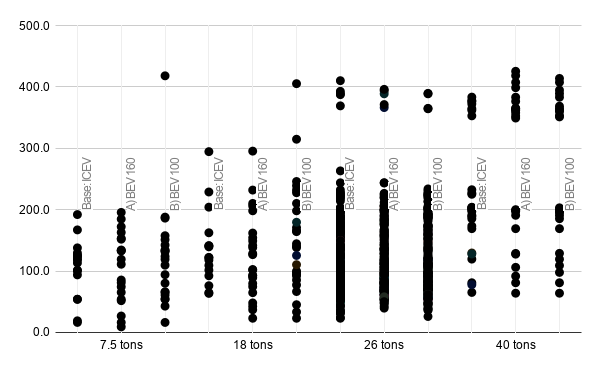
\includegraphics[width=\textwidth]{elektrifizierung/ersetzung1zu1/figs/tourDistances_total_160-100.png}
		\caption{Observed daily tour distances [km] driven by vehicle type and case.}%
		\label{fig:tourDistances}
	\end{minipage}%
	\begin{minipage}{.5\textwidth}
		\centering
		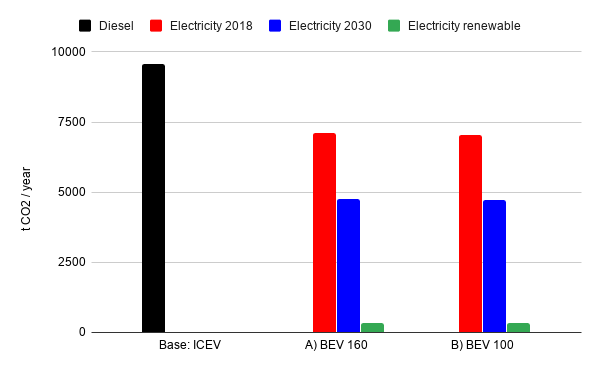
\includegraphics[width=\textwidth]{elektrifizierung/ersetzung1zu1/figs//CO2-Emissions.png}
		\caption{Calculated CO2 emissions per year.}%
		\label{fig:CO2Emssions}
	\end{minipage}
\end{figure}


\section{Conclusion and Outlook}
\label{sec:conclusion}
In this paper, we analysed whether electrification is suitable for the urban last mile supply of shops based on a case study in the city of Berlin. The BEVs were designed to have the same payload as ICEVs in the same weight class.
In the selected scenarios we could show with an ex-post analysis that 56\% percent of the resulting tours can be driven with battery electric trucks without recharging during the tour, another 34\% with recharging one time.

In terms of costs, the change from ICEVs to BEVs will result in increasing costs by 23\% if the chassis of the BEVs are 60\% more expensive as the chassis of the ICEVs (case A). In the sensitivity case (B) with equal chassis cost, the total transportation costs will increase by 17\%. These costs include the costs for the battery as well as the costs for diesel respectively electric energy. 
Regarding the fleet size and composition, no significant change is observed. 

Using BEVs for all tours leads to a reduction of 2\,500 to 9\,200 t GHG per year depending on the assumed electricity production. This is a reduction by 26 to 96\% compared to the usage of ICEVs.

In this paper we evaluate the feasibility of using BEVs with an ex-post analysis. Including a vehicle type specific distance constraint into the VRP can force respecting this limitation already in the tour generation. 
Based on this, including (re-)charging into the VRP solving may be a useful further development. It may also force to replan the logistics network introducing additional hubs between the depots and the shops.
Providing additional variants of vehicles with larger battery capacity is another option, even though this leads to a reduction of the payload. 
Regardless of these improvement potentials for our method, we were able to show that even without major changes in the carriers operating strategies, a significant amount of urban freight delivery tours can be electrified with current technology.

%%%%%%%%%%%%%%%%%%%%%%%%%%%%
%%%%%%%%%%%%%%%%%%%%%%%%%%%%
